\documentclass{standalone}
\usepackage{amsmath}
\usepackage[T1]{fontenc}
\usepackage[utf8]{inputenc}

\usepackage[usenames,dvipsnames]{xcolor}

\usepackage{tikz}
\usetikzlibrary{arrows, shapes, matrix}

\begin{document}

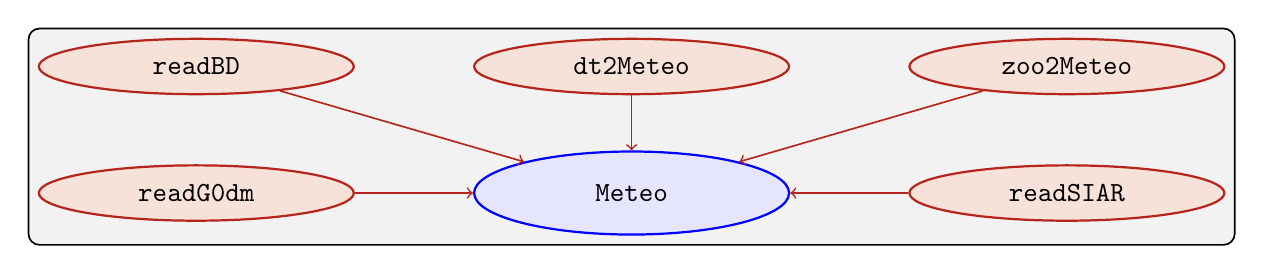
\begin{tikzpicture}[auto,
  method/.style={rectangle, rounded corners, draw=black, thick, fill=gray!30,
    minimum height = 3em, align=flush center, inner sep=1pt},
  %
  function/.style ={draw=BrickRed, thick, ellipse, fill=BrickRed!10,
    minimum height=2em},
  % 
  class/.style ={draw=Blue, thick, ellipse, fill=Blue!10,
    minimum height=3em},
  %
  utils/.style ={draw=Green, thick, ellipse, fill=Green!10,
    minimum height=2em},
  %
  simple/.style ={draw=black!50, thick, ellipse, fill=white}
  ]
  
  \tikzset{every path/.style={line width=.6pt}}

  \begin{scope}
    \matrix [matrix of nodes, rounded corners, fill=gray!10, draw=black, column
  sep=15mm,row sep=7mm, minimum width=4cm] (Meteo) {
    %%%%%%%%%%%%%%%%%%%%%%%%%%%%%%% 
    \node [function] (readBD) {\texttt{readBD}}; &
    \node [function] (dt2Meteo) {\texttt{dt2Meteo}}; &
    \node [function] (zoo2Meteo) {\texttt{zoo2Meteo}}; \\
    %%%%%%%%%%%%%%%%%%%%%%%%%%%%%%%
    \node [function] (readG0dm) {\texttt{readG0dm}}; &
    \node [class] (meteo) {\texttt{Meteo}}; &
    \node [function] (readSIAR) {\texttt{readSIAR}}; \\
    %%%%%%%%%%%%%%%%%%%%%%%%%%%%%%%
  };
\end{scope}

\begin{scope}
  \draw [->, BrickRed] (readG0dm) -- (meteo);
  \draw [->, BrickRed] (readBD) -- (meteo);
  \draw [->, BrickRed] (dt2Meteo) -- (meteo);
  \draw [->, BrickRed] (zoo2Meteo) -- (meteo);
  \draw [->, BrickRed] (readSIAR) -- (meteo);
\end{scope}
  
\end{tikzpicture}

\end{document}
